\chapter{Einleitung}
In der heutigen Zeit gibt es viele interessante Gadgets, die unterschiedlichste Daten liefern. Seien das Pulsmesser, Heizungsregler oder das Multimediasystem zu Hause, diese Technologien lassen sich auch für den Fahrradfahrer nutzen. Es gibt bereits sogenannte Fahrradcomputer, welche die Geschwindigkeit messen und über ein separates Display ausgeben, jedoch werden die meisten mit einer Batterie betrieben, deren Laufzeit begrenzt ist. Mit der Möglichkeit des Energy Harvesting wird die Batterie und deren begrenzte Laufzeit gänzlich ersetzt. Bluetooth Low Energy kann Daten mit sehr wenig Energie übertragen, damit können die Daten, wie Geschwindigkeit oder Höhenmeter, an ein Android-Endgerät übermittelt werden.


\section{Ausgangslage}



Zwei Nachteile: Batteriewechsel und zusätzliches Display. Ein Handy hat jeder. Deshalb diese zur Anzeige benutzen.


Nennen, was in dieser Arbeit \textbf{neu} erarbeitet wird.
...



Als Grundlage für die Arbeit gibt es einen Aufbau aus der Machbarkeitsstudie "Bicycle computer and sensoric powered with harvested energy" (\cite{PA_bicycle}), welche als Projektarbeit im Herbstsemester 2015 beim Institut of Embedded Systems an der ZHAW erarbeitet wurde. Das Ergebnis ist ein Fahrrad, an welchem ein einfacher Aufbau befestigt ist. Die Anfertigung der Machbarkeitsstudie funktioniert bei hohen Geschwindigkeiten relativ zuverlässig, jedoch ist die Energie bei Geschwindigkeiten eines normalen Radfahrers nicht zu erreichen. Die Übertragung der gemessenen Geschwindigkeit funktioniert über Bluetooth Smart, sofern die Energie welche über Bewegungsinduktion erzeugt wird, für eine Kommunikation ausreicht. In der Machbarkeitsstudie wurde der Beweis erbracht, dass durch Bewegungsinduktion genug Energie erzeugt werden kann, um die Geschwindigkeit des Fahrrads, welche über die Detektion eines Magnets an den Speichen des Fahrrads ermittelt wird, per Bluetooth Smart zu übermitteln.\\

Es gibt bereits Fahrradcomputer von namentlichen Herstellern wie SIGMA SPORT, jedoch werden alle Geräte mit einer Batterie betrieben. Der aktuelle Ladestand der Batterie wird bei vielen Produkten angezeigt und am Fahrradcomputer ist auch der Ladestand der einzelnen Sensoren zu sehen. Die Position wird mittels GPS ermittelt und kann am Computer ausgelesen werden. Der Hersteller POLAR stellt ein Gerät her, welches die Fahrt über GPS aufzeichnet und wichtige Informationen zur Trainingsverbesserung liefert. Bisher ist auf dem Markt kein Gerät vorhanden, welches ohne Batterie funktioniert. Alle Geräte müssen nach spätestens 1-2 Jahren gewartet werden, das heisst das Gerät muss demontiert werden.\\

%(Zweiter Nachteil: Externes Display. Wir benutzen ein Handy, das jeder hat.)\\

Der Hersteller Reelight stellt keine Fahrradcomputer her, jedoch hat er eine interessante Methode, um Energie beim Fahrrad zu gewinnen. Es werden Wirbelströme zur Energieerzeugung genutzt, das genaue Prinzip wird auf der Homepage nicht erklärt. Die erzeugte Energie wird bei dem Produkt City Supreme von Reelight über eine LED in Licht umgewandelt und so als Lampe für das Fahrrad benutzt. Bei der Benutzung fühlt man, dass sich im Innern der Lampe etwas bewegt. Unserer Meinung nach ist ein Magnet so gelagert, dass er sich drehen kann. Der Magnet (produziert auf der Felge ein Magnetfeld??) durchsetzt die Felge des Fahrrads mit einem Magnetfeld, was Wirbelströme erzeugt und ein Magnetfeld, welches dem des Magneten im Produkt entgegenwirkt. Die Lagerung des Magneten erlaubt ihm jetzt sich zu drehen, so dass das Magnetfeld, welches die Felge durchsetzt sich ändert und wieder ein Magnetfeld erzeugt, dass den Magneten bewegt. Die Vermutung liegt nahe, dass um den Magneten eine Spule positioniert ist, durch die Bewegung des Magneten wird dann eine Spannung in der Spule induziert und die LED kann betrieben werden.\\

Die aktuellen Fahrradcomputer auf dem Markt müssen spätestens nach 1 - 2 Jahren gewartet werden, das heisst es muss die Batterie ausgetauscht werden. Eine Verbesserung wäre es, wenn man den Fahrradcomputer nicht mit einer Batterie betreiben würde, sondern wenn die Energie aus der Umwelt bzw. dem Fahrrad gewonnen werden könnte. Es gibt bereits den Dynamo, jedoch bremst dieser das Rad merklich ab und ist meistens nicht geräuscharm. Die Möglichkeit vom Hersteller Reelight, die Energie über Wirbelströme zu erzeugen, wäre eine interessante Idee jedoch benötigt das bewegliche Teile, welche problematisch sind, dass diese nach einigen Jahren evtl. nicht mehr richtig funktionieren und ausgewechselt werden müssen. Aufgrund der oben genannten Punkten wurde eine Aufgabenstellung für die Entwicklung eines Fahrradcomputers erstellt, welche über Energy Harvesting funktioniert. Die Arbeit soll auf der vorangegangenen Machbarkeitsstudie aufbauen.


\section{Definition der Aufgabenstellung}
In der Ausschreibung der Arbeit ist der Inhalt der Bachelorarbeit zusammengefasst (siehe \ref{anhang_ausschreibung}). Das Ziel der Arbeit besteht darin, einen bestehenden Prototypen eines batterielosen Fahrradcomputers zu verbessern und zu optimieren. Die bestehende Hardware soll optimiert und bestenfalls verkleinert werden. Weiter soll eine App für ein Android-Endgerät entwickelt werden, in der die Messwerte dargestellt werden.

Aus den Themen entstand eine Aufgabenstellung mit folgenden Punkten:


% [label={\alph*)}]
\begin{enumerate} 

\item Inbetriebnahme des Prototypen, Einlesen in die vorangegangene Projektarbeit und Beschäftigung mit der Materie, sind die Hauptpunkte des ersten Schrittes.

\item Die bestehende Hardware muss verkleinert und überarbeitet werden. Dafür wird ein neues PCB entworfen, welches verschiedene vorhandene Platinen vereint.

\item Initialisierung der Bluetooth-Schnittstelle muss auf dem Android-Endgerät und der Hardware vorgenommen werden. Eine erste Bluetooth-Kommunikation zwischen der Hardware und der Applikationen ist implementiert.

\item Das bestehende Energiemanagement soll auf die Anwendung eines Fahrradcomputers optimiert werden.

\item Die Benutzeroberfläche der Android-Applikation soll benutzerfreundlich und optisch ansprechend gestaltet werden.

\item Die erfassten Messwerte der Geschwindigkeit und der aktuellen Höhe sollen über Bluetooth übermittelt werden.

\item	Die erfassten Daten sollen gespeichert und nur dann übertragen werden, wenn die nötige Energie vorhanden ist.

\item	Per GPS soll die aktuelle Position ermittelt, sowie die bereits abgefahrene Route erfasst werden. Alles soll auf einer Karte veranschaulicht werden.

\item	Die Beschleunigung, Luftfeuchtigkeit und Temperatur sollen ebenfalls erfasst und über Bluetooth übermittelt werden.


\item	Das Energiemanagement soll für verschiedene Geschwindigkeiten optimiert werden.
\end{enumerate}

Für diese Bachelorarbeit sind die Punkte a) bis f) als Minimalanforderungen zu verstehen, während sich die Punkte f) bis j) dynamisch und in Abhängigkeit des Projektfortschritts gestalten lassen.\\

Aus diesen Anforderungen entstand der im Anhang \ref{anhang_projektplan} abgelegte Projektplan.

\section{Übersicht der Aufgabenblöcke}
Aus der Aufgabenstellung sind folgende Arbeitsblöcke (siehe Abbildung \ref{arbeitsbloecke} ) entstanden. Die gepunkteten Blöcke sind optional, die voll umrandeten das Minimum. Die Projektplanung ist so aufgebaut, dass bei Meilenstein 1, das Layout gezeichnet ist, bei Meilenstein 2 die Kommunikation zur App besteht, bei Meilenstein 3 die überarbeitete Version des Prototyps gezeigt wird und bis dahin das Minimum erreicht ist. Welche optionalen Ziele realisiert werden, wird im Meilenstein 3 definiert. Der Projektplan findet sich im Anhang \ref{anhang_projektplan}.

\begin{figure}[h]
    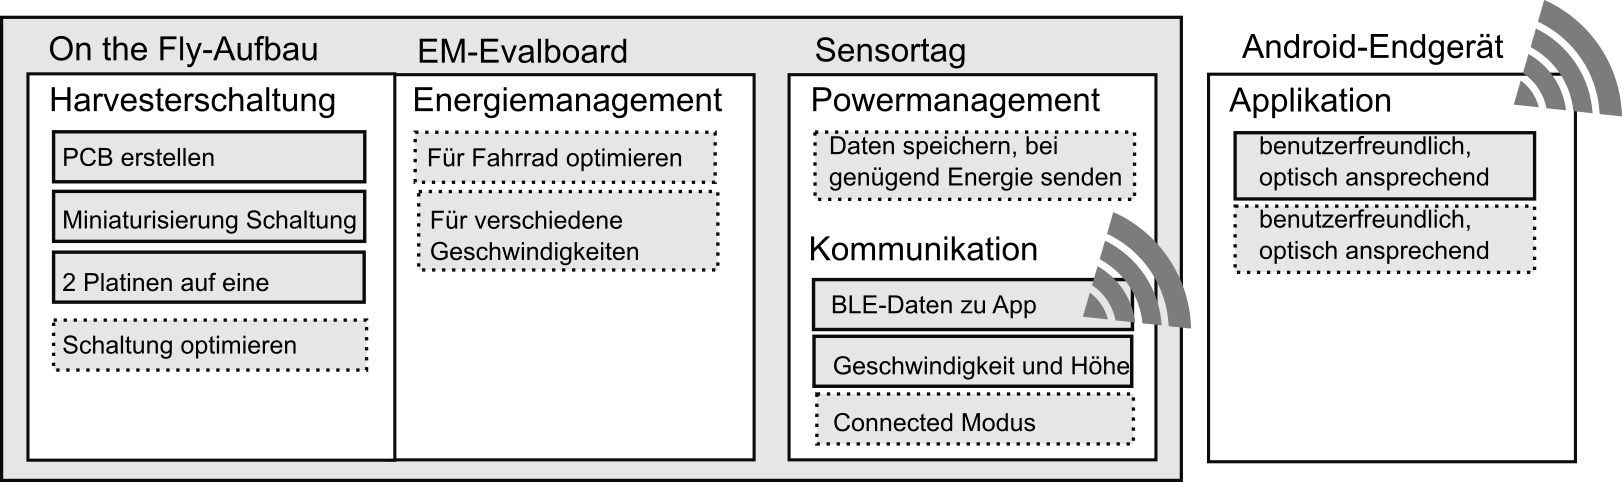
\includegraphics[width=15cm]{../ressources/Projektorganisation/Arbeitsbloecke.png} 
    \caption{Arbeitsblöcke}
\end{figure}\label{arbeitsbloecke} 

